\documentclass[twoside]{book}

% Packages required by doxygen
\usepackage{fixltx2e}
\usepackage{calc}
\usepackage{doxygen}
\usepackage[export]{adjustbox} % also loads graphicx
\usepackage{graphicx}
\usepackage[utf8]{inputenc}
\usepackage{makeidx}
\usepackage{multicol}
\usepackage{multirow}
\PassOptionsToPackage{warn}{textcomp}
\usepackage{textcomp}
\usepackage[nointegrals]{wasysym}
\usepackage[table]{xcolor}

% Font selection
\usepackage[T1]{fontenc}
\usepackage[scaled=.90]{helvet}
\usepackage{courier}
\usepackage{amssymb}
\usepackage{sectsty}
\renewcommand{\familydefault}{\sfdefault}
\allsectionsfont{%
  \fontseries{bc}\selectfont%
  \color{darkgray}%
}
\renewcommand{\DoxyLabelFont}{%
  \fontseries{bc}\selectfont%
  \color{darkgray}%
}
\newcommand{\+}{\discretionary{\mbox{\scriptsize$\hookleftarrow$}}{}{}}

% Page & text layout
\usepackage{geometry}
\geometry{%
  a4paper,%
  top=2.5cm,%
  bottom=2.5cm,%
  left=2.5cm,%
  right=2.5cm%
}
\tolerance=750
\hfuzz=15pt
\hbadness=750
\setlength{\emergencystretch}{15pt}
\setlength{\parindent}{0cm}
\setlength{\parskip}{3ex plus 2ex minus 2ex}
\makeatletter
\renewcommand{\paragraph}{%
  \@startsection{paragraph}{4}{0ex}{-1.0ex}{1.0ex}{%
    \normalfont\normalsize\bfseries\SS@parafont%
  }%
}
\renewcommand{\subparagraph}{%
  \@startsection{subparagraph}{5}{0ex}{-1.0ex}{1.0ex}{%
    \normalfont\normalsize\bfseries\SS@subparafont%
  }%
}
\makeatother

% Headers & footers
\usepackage{fancyhdr}
\pagestyle{fancyplain}
\fancyhead[LE]{\fancyplain{}{\bfseries\thepage}}
\fancyhead[CE]{\fancyplain{}{}}
\fancyhead[RE]{\fancyplain{}{\bfseries\leftmark}}
\fancyhead[LO]{\fancyplain{}{\bfseries\rightmark}}
\fancyhead[CO]{\fancyplain{}{}}
\fancyhead[RO]{\fancyplain{}{\bfseries\thepage}}
\fancyfoot[LE]{\fancyplain{}{}}
\fancyfoot[CE]{\fancyplain{}{}}
\fancyfoot[RE]{\fancyplain{}{\bfseries\scriptsize Generated by Doxygen }}
\fancyfoot[LO]{\fancyplain{}{\bfseries\scriptsize Generated by Doxygen }}
\fancyfoot[CO]{\fancyplain{}{}}
\fancyfoot[RO]{\fancyplain{}{}}
\renewcommand{\footrulewidth}{0.4pt}
\renewcommand{\chaptermark}[1]{%
  \markboth{#1}{}%
}
\renewcommand{\sectionmark}[1]{%
  \markright{\thesection\ #1}%
}

% Indices & bibliography
\usepackage{natbib}
\usepackage[titles]{tocloft}
\setcounter{tocdepth}{3}
\setcounter{secnumdepth}{5}
\makeindex

% Hyperlinks (required, but should be loaded last)
\usepackage{ifpdf}
\ifpdf
  \usepackage[pdftex,pagebackref=true]{hyperref}
\else
  \usepackage[ps2pdf,pagebackref=true]{hyperref}
\fi
\hypersetup{%
  colorlinks=true,%
  linkcolor=blue,%
  citecolor=blue,%
  unicode%
}

% Custom commands
\newcommand{\clearemptydoublepage}{%
  \newpage{\pagestyle{empty}\cleardoublepage}%
}

\usepackage{caption}
\captionsetup{labelsep=space,justification=centering,font={bf},singlelinecheck=off,skip=4pt,position=top}

%===== C O N T E N T S =====

\usepackage{CJKutf8}
\begin {document}
\begin{CJK}{UTF8}{gbsn}


% Titlepage & ToC
\hypersetup{pageanchor=false,
             bookmarksnumbered=true,
             pdfencoding=unicode
            }
\pagenumbering{roman}
\begin{titlepage}
\vspace*{7cm}
\begin{center}%
{\Large My Project }\\
\vspace*{1cm}
{\large Generated by Doxygen 1.8.11}\\
\end{center}
\end{titlepage}
\clearemptydoublepage
\tableofcontents
\clearemptydoublepage
\pagenumbering{arabic}
\hypersetup{pageanchor=true}

%--- Begin generated contents ---
\chapter{Class Index}
\section{Class List}
Here are the classes, structs, unions and interfaces with brief descriptions\+:\begin{DoxyCompactList}
\item\contentsline{section}{\hyperlink{classhw3}{hw3} }{\pageref{classhw3}}{}
\end{DoxyCompactList}

\chapter{File Index}
\section{File List}
Here is a list of all documented files with brief descriptions\+:\begin{DoxyCompactList}
\item\contentsline{section}{\hyperlink{hw3_8cpp}{hw3.\+cpp} \\*函数实现 }{\pageref{hw3_8cpp}}{}
\item\contentsline{section}{\hyperlink{hw3_8h}{hw3.\+h} }{\pageref{hw3_8h}}{}
\item\contentsline{section}{\hyperlink{main_8cpp}{main.\+cpp} }{\pageref{main_8cpp}}{}
\end{DoxyCompactList}

\chapter{Class Documentation}
\hypertarget{classhw3}{}\section{hw3 Class Reference}
\label{classhw3}\index{hw3@{hw3}}
\subsection*{Public Member Functions}
\begin{DoxyCompactItemize}
\item 
void \hyperlink{classhw3_acdd257e9849222197ea2802daff7235b}{set\+\_\+size} (int)
\begin{DoxyCompactList}\small\item\em 设置进程数目 \end{DoxyCompactList}\item 
void \hyperlink{classhw3_a1f277d537a9091e40bf34ca6b1f1f133}{set\+\_\+rank} (int)
\begin{DoxyCompactList}\small\item\em 设置进程编号 \end{DoxyCompactList}\item 
void \hyperlink{classhw3_af0e7bc760ae9e229d6fb5d4e31175010}{set\+\_\+f} (const R\+HS \&)
\begin{DoxyCompactList}\small\item\em 设置右端项 \end{DoxyCompactList}\item 
void \hyperlink{classhw3_a0acf7fc706e4711d13fe1656d9391f5a}{set\+\_\+N} (int)
\begin{DoxyCompactList}\small\item\em 设置网格密度 \end{DoxyCompactList}\item 
void \hyperlink{classhw3_a7ff2691e20e38b4dbedb0fe71578bfd4}{set\+\_\+lambda} (double)
\begin{DoxyCompactList}\small\item\em 设置lambda参数 \end{DoxyCompactList}\item 
void \hyperlink{classhw3_a2a474121810abd2e4b455892c0e96a84}{set\+\_\+step} (int)
\begin{DoxyCompactList}\small\item\em 设置迭代步数 \end{DoxyCompactList}\item 
S\+OL \hyperlink{classhw3_aff03f6d8dad50d226cd493c1789790fe}{solve} ()
\begin{DoxyCompactList}\small\item\em 求解 \end{DoxyCompactList}\item 
void \hyperlink{classhw3_af267c71c8058aba6c710c213e412a7aa}{set\+\_\+solution} (const R\+HS \&)
\begin{DoxyCompactList}\small\item\em 设置真解 \end{DoxyCompactList}\item 
double \hyperlink{classhw3_a84140f8e9e076437b44108f96ec85384}{error} ()
\begin{DoxyCompactList}\small\item\em 设置误差 \end{DoxyCompactList}\end{DoxyCompactItemize}


\subsection{Member Function Documentation}
\index{hw3@{hw3}!error@{error}}
\index{error@{error}!hw3@{hw3}}
\subsubsection[{\texorpdfstring{error()}{error()}}]{\setlength{\rightskip}{0pt plus 5cm}double hw3\+::error (
\begin{DoxyParamCaption}
{}
\end{DoxyParamCaption}
)}\hypertarget{classhw3_a84140f8e9e076437b44108f96ec85384}{}\label{classhw3_a84140f8e9e076437b44108f96ec85384}


设置误差 

\begin{DoxyReturn}{Returns}
误差 
\end{DoxyReturn}
\index{hw3@{hw3}!set\+\_\+f@{set\+\_\+f}}
\index{set\+\_\+f@{set\+\_\+f}!hw3@{hw3}}
\subsubsection[{\texorpdfstring{set\+\_\+f(const R\+H\+S \&)}{set_f(const RHS &)}}]{\setlength{\rightskip}{0pt plus 5cm}void hw3\+::set\+\_\+f (
\begin{DoxyParamCaption}
\item[{const R\+HS \&}]{f1}
\end{DoxyParamCaption}
)}\hypertarget{classhw3_af0e7bc760ae9e229d6fb5d4e31175010}{}\label{classhw3_af0e7bc760ae9e229d6fb5d4e31175010}


设置右端项 


\begin{DoxyParams}{Parameters}
{\em R\+HS} & 右端项函数\\
\hline
{\em f1} & 右端项 \\
\hline
\end{DoxyParams}
\index{hw3@{hw3}!set\+\_\+lambda@{set\+\_\+lambda}}
\index{set\+\_\+lambda@{set\+\_\+lambda}!hw3@{hw3}}
\subsubsection[{\texorpdfstring{set\+\_\+lambda(double)}{set_lambda(double)}}]{\setlength{\rightskip}{0pt plus 5cm}void hw3\+::set\+\_\+lambda (
\begin{DoxyParamCaption}
\item[{double}]{lambda1}
\end{DoxyParamCaption}
)}\hypertarget{classhw3_a7ff2691e20e38b4dbedb0fe71578bfd4}{}\label{classhw3_a7ff2691e20e38b4dbedb0fe71578bfd4}


设置lambda参数 

设置参数lambda


\begin{DoxyParams}{Parameters}
{\em double} & lambda\\
\hline
{\em lambda1} & 参数lambda \\
\hline
\end{DoxyParams}
\index{hw3@{hw3}!set\+\_\+N@{set\+\_\+N}}
\index{set\+\_\+N@{set\+\_\+N}!hw3@{hw3}}
\subsubsection[{\texorpdfstring{set\+\_\+\+N(int)}{set_N(int)}}]{\setlength{\rightskip}{0pt plus 5cm}void hw3\+::set\+\_\+N (
\begin{DoxyParamCaption}
\item[{int}]{N1}
\end{DoxyParamCaption}
)}\hypertarget{classhw3_a0acf7fc706e4711d13fe1656d9391f5a}{}\label{classhw3_a0acf7fc706e4711d13fe1656d9391f5a}


设置网格密度 

设置网格数目


\begin{DoxyParams}{Parameters}
{\em int} & 网格密度\\
\hline
{\em N1} & 网格数目 \\
\hline
\end{DoxyParams}
\index{hw3@{hw3}!set\+\_\+rank@{set\+\_\+rank}}
\index{set\+\_\+rank@{set\+\_\+rank}!hw3@{hw3}}
\subsubsection[{\texorpdfstring{set\+\_\+rank(int)}{set_rank(int)}}]{\setlength{\rightskip}{0pt plus 5cm}void hw3\+::set\+\_\+rank (
\begin{DoxyParamCaption}
\item[{int}]{rank1}
\end{DoxyParamCaption}
)}\hypertarget{classhw3_a1f277d537a9091e40bf34ca6b1f1f133}{}\label{classhw3_a1f277d537a9091e40bf34ca6b1f1f133}


设置进程编号 


\begin{DoxyParams}{Parameters}
{\em int} & 进程编号\\
\hline
{\em rank1} & 进程编号 \\
\hline
\end{DoxyParams}
\index{hw3@{hw3}!set\+\_\+size@{set\+\_\+size}}
\index{set\+\_\+size@{set\+\_\+size}!hw3@{hw3}}
\subsubsection[{\texorpdfstring{set\+\_\+size(int)}{set_size(int)}}]{\setlength{\rightskip}{0pt plus 5cm}void hw3\+::set\+\_\+size (
\begin{DoxyParamCaption}
\item[{int}]{size1}
\end{DoxyParamCaption}
)}\hypertarget{classhw3_acdd257e9849222197ea2802daff7235b}{}\label{classhw3_acdd257e9849222197ea2802daff7235b}


设置进程数目 


\begin{DoxyParams}{Parameters}
{\em 进程数目} & \\
\hline
{\em size1} & 进程数目 \\
\hline
\end{DoxyParams}
\index{hw3@{hw3}!set\+\_\+solution@{set\+\_\+solution}}
\index{set\+\_\+solution@{set\+\_\+solution}!hw3@{hw3}}
\subsubsection[{\texorpdfstring{set\+\_\+solution(const R\+H\+S \&)}{set_solution(const RHS &)}}]{\setlength{\rightskip}{0pt plus 5cm}void hw3\+::set\+\_\+solution (
\begin{DoxyParamCaption}
\item[{const R\+HS \&}]{u1}
\end{DoxyParamCaption}
)}\hypertarget{classhw3_af267c71c8058aba6c710c213e412a7aa}{}\label{classhw3_af267c71c8058aba6c710c213e412a7aa}


设置真解 

设置真解(供测试使用)


\begin{DoxyParams}{Parameters}
{\em R\+HS} & 真解\\
\hline
{\em u1} & 真解 \\
\hline
\end{DoxyParams}
\index{hw3@{hw3}!set\+\_\+step@{set\+\_\+step}}
\index{set\+\_\+step@{set\+\_\+step}!hw3@{hw3}}
\subsubsection[{\texorpdfstring{set\+\_\+step(int)}{set_step(int)}}]{\setlength{\rightskip}{0pt plus 5cm}void hw3\+::set\+\_\+step (
\begin{DoxyParamCaption}
\item[{int}]{step1}
\end{DoxyParamCaption}
)}\hypertarget{classhw3_a2a474121810abd2e4b455892c0e96a84}{}\label{classhw3_a2a474121810abd2e4b455892c0e96a84}


设置迭代步数 


\begin{DoxyParams}{Parameters}
{\em int} & 迭代步数\\
\hline
{\em step1} & 迭代步数 \\
\hline
\end{DoxyParams}
\index{hw3@{hw3}!solve@{solve}}
\index{solve@{solve}!hw3@{hw3}}
\subsubsection[{\texorpdfstring{solve()}{solve()}}]{\setlength{\rightskip}{0pt plus 5cm}std\+::vector$<$ std\+::complex$<$ double $>$ $>$ hw3\+::solve (
\begin{DoxyParamCaption}
{}
\end{DoxyParamCaption}
)}\hypertarget{classhw3_aff03f6d8dad50d226cd493c1789790fe}{}\label{classhw3_aff03f6d8dad50d226cd493c1789790fe}


求解 

\begin{DoxyReturn}{Returns}
解 
\end{DoxyReturn}


The documentation for this class was generated from the following files\+:\begin{DoxyCompactItemize}
\item 
\hyperlink{hw3_8h}{hw3.\+h}\item 
\hyperlink{hw3_8cpp}{hw3.\+cpp}\end{DoxyCompactItemize}

\chapter{File Documentation}
\hypertarget{hw3_8cpp}{}\section{hw3.\+cpp File Reference}
\label{hw3_8cpp}\index{hw3.\+cpp@{hw3.\+cpp}}


函数实现  


{\ttfamily \#include \char`\"{}hw3.\+h\char`\"{}}\\*
Include dependency graph for hw3.\+cpp\+:\nopagebreak
\begin{figure}[H]
\begin{center}
\leavevmode
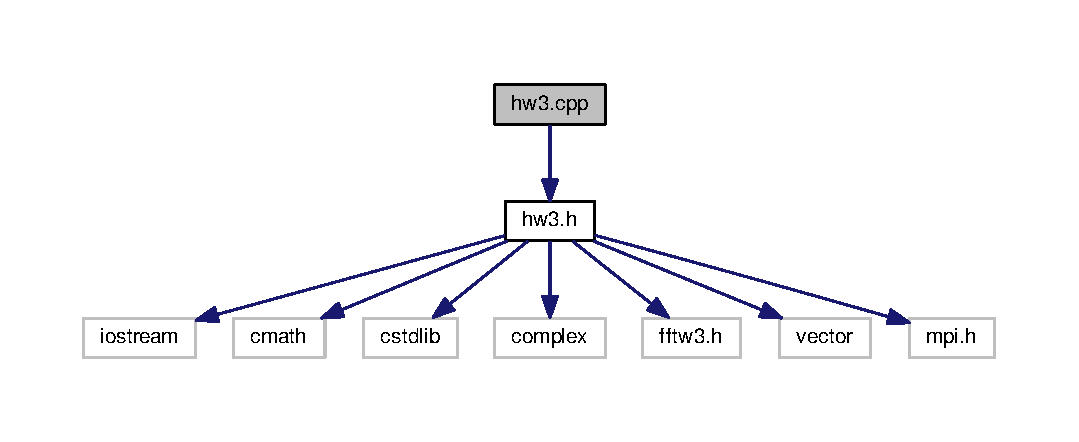
\includegraphics[width=350pt]{hw3_8cpp__incl}
\end{center}
\end{figure}


\subsection{Detailed Description}
函数实现 

\begin{DoxyAuthor}{Author}
lczheng, \href{mailto:lczheng@pku.edu.cn}{\tt lczheng@pku.\+edu.\+cn}
\end{DoxyAuthor}
\begin{DoxyDate}{Date}
2016-\/12-\/10 
\end{DoxyDate}

\hypertarget{hw3_8h}{}\section{hw3.\+h File Reference}
\label{hw3_8h}\index{hw3.\+h@{hw3.\+h}}
{\ttfamily \#include $<$iostream$>$}\\*
{\ttfamily \#include $<$cmath$>$}\\*
{\ttfamily \#include $<$cstdlib$>$}\\*
{\ttfamily \#include $<$complex$>$}\\*
{\ttfamily \#include $<$fftw3.\+h$>$}\\*
{\ttfamily \#include $<$vector$>$}\\*
{\ttfamily \#include \char`\"{}mpi.\+h\char`\"{}}\\*
Include dependency graph for hw3.\+h\+:\nopagebreak
\begin{figure}[H]
\begin{center}
\leavevmode
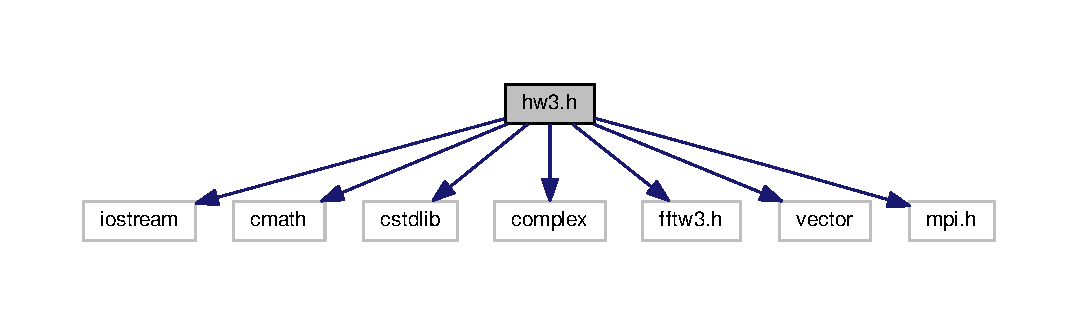
\includegraphics[width=350pt]{hw3_8h__incl}
\end{center}
\end{figure}
This graph shows which files directly or indirectly include this file\+:\nopagebreak
\begin{figure}[H]
\begin{center}
\leavevmode
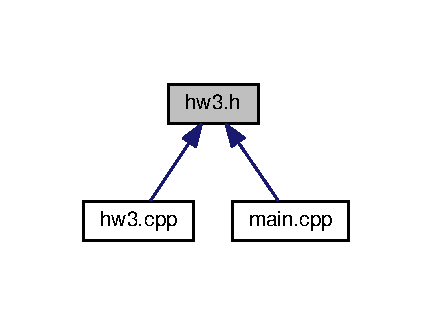
\includegraphics[width=208pt]{hw3_8h__dep__incl}
\end{center}
\end{figure}
\subsection*{Classes}
\begin{DoxyCompactItemize}
\item 
class \hyperlink{classhw3}{hw3}
\end{DoxyCompactItemize}


\subsection{Detailed Description}
\begin{DoxyAuthor}{Author}
lczheng, \href{mailto:lczheng@pku.edu.cn}{\tt lczheng@pku.\+edu.\+cn}
\end{DoxyAuthor}
\begin{DoxyDate}{Date}
2016-\/11-\/27 
\end{DoxyDate}

\hypertarget{main_8cpp}{}\section{main.\+cpp File Reference}
\label{main_8cpp}\index{main.\+cpp@{main.\+cpp}}
{\ttfamily \#include \char`\"{}Heat.\+h\char`\"{}}\\*
Include dependency graph for main.\+cpp\+:
\nopagebreak
\begin{figure}[H]
\begin{center}
\leavevmode
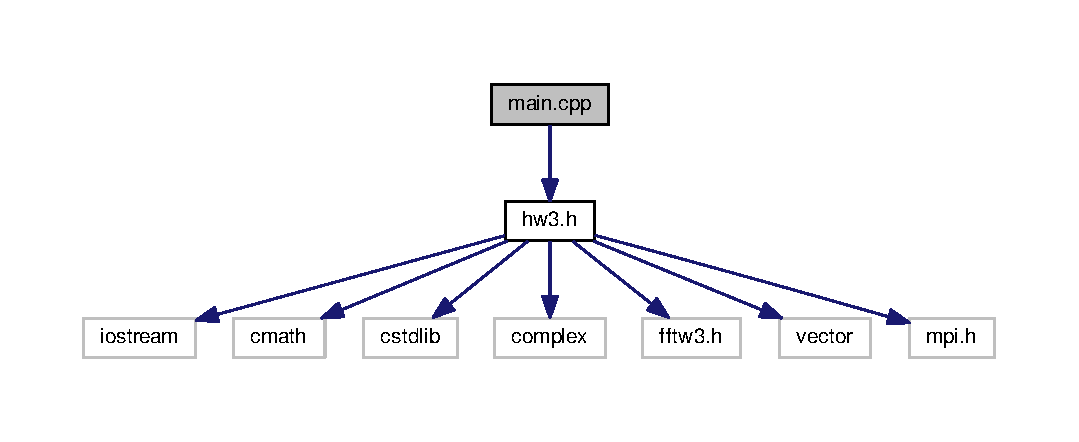
\includegraphics[width=350pt]{main_8cpp__incl}
\end{center}
\end{figure}
\subsection*{Functions}
\begin{DoxyCompactItemize}
\item 
double {\bfseries u} (double x, double y, double z, double t)\hypertarget{main_8cpp_a7f946b7182f074fdec4cd02cceec0f95}{}\label{main_8cpp_a7f946b7182f074fdec4cd02cceec0f95}

\item 
double {\bfseries f} (double x, double y, double z, double t)\hypertarget{main_8cpp_a2cb048afa8f6f33ffe18db917a6164b0}{}\label{main_8cpp_a2cb048afa8f6f33ffe18db917a6164b0}

\item 
double {\bfseries u0} (double x, double y, double z)\hypertarget{main_8cpp_a50b8caccf6e7fea0ad0cf221da153050}{}\label{main_8cpp_a50b8caccf6e7fea0ad0cf221da153050}

\item 
double {\bfseries g\+\_\+up} (double x, double y, double z, double t)\hypertarget{main_8cpp_a24122920a607797e7ee374ea86e07f26}{}\label{main_8cpp_a24122920a607797e7ee374ea86e07f26}

\item 
double {\bfseries g\+\_\+down} (double x, double y, double z, double t)\hypertarget{main_8cpp_a76d374eeb92bbd16ef04a38748906749}{}\label{main_8cpp_a76d374eeb92bbd16ef04a38748906749}

\item 
int {\bfseries transform} (int i, int j, int k, int N)\hypertarget{main_8cpp_a2ea6b0858e6766287931140dcb973820}{}\label{main_8cpp_a2ea6b0858e6766287931140dcb973820}

\item 
int {\bfseries main} (int argc, char $\ast$argv\mbox{[}$\,$\mbox{]})\hypertarget{main_8cpp_a0ddf1224851353fc92bfbff6f499fa97}{}\label{main_8cpp_a0ddf1224851353fc92bfbff6f499fa97}

\end{DoxyCompactItemize}


\subsection{Detailed Description}
\begin{DoxyAuthor}{Author}
lczheng, \href{mailto:lczheng@pku.edu.cn}{\tt lczheng@pku.\+edu.\+cn}
\end{DoxyAuthor}
\begin{DoxyDate}{Date}
2016-\/12-\/31 
\end{DoxyDate}

%--- End generated contents ---

% Index
\backmatter
\newpage
\phantomsection
\clearemptydoublepage
\addcontentsline{toc}{chapter}{Index}
\printindex

\end{CJK}
\end {document}
